\chapter{相关概念}
	\label{chapter_concepts}
	本章介绍论文中涉及到的相关概念及其背景知识,主要包含云服务中的QoS属性,云服务中的QoS预测问题,基于协同过滤的QoS预测方法,()。
	\section{云服务中的QoS属性}
	\label{sec_QoS_attributes}
	云计算近年来备受关注。云计算已经成为一个可扩展的服务消费和交付平台。云服务是云计算在用户端的表达,继承了云计算的特点。云服务不仅要满足用户的功能性需求外,还要满足QoS约束。
	
	服务质量(QoS)现已广泛运用在测量和评价系统或服务的非功能性特点的指标。QoS是可以从多个方面对系统或服务进行衡量,故具有多个属性指标,我们可以简单的归为两类。一类是用户相关属性,比如说价格(price),流行度(popularity)等;另一类是非用户相关属性,像响应时间(response-time),吞吐量(throughput)等。
	
	监测云服务QoS性能工作通常可以在云服务提供商一端进行,亦或也能在基于用户的角度进行观察。
	
		\subsection{响应时间(response-time)}
		\label{sec_response-time}
		响应时间是一项云服务去响应请求所花费的总时间也称为延迟时间(latency time),其中所主要构成包括网络往返时间(Network Round Trip Time,简写为Network RTT),重新传输时间(Retransmission Time,简写为Retrans),数据传输时间(Data Transfer Time,简写为Data Xfer)以及服务器响应时间(Server Response Time,简写为Server Resp)。所以,可以用公式 \ref{eq_compute_response-time}将QoS响应时间属性形式化表示。
		\begin{equation}
			response-time=NetworkRTT+Retrans+DataXfer+ServerResp
			\label{eq_compute_response-time}
		\end{equation}
		\subsection{吞吐量(Throughput)}
		\label{sec_throughput}
		吞吐量是指云服务在单位时间内成功处理请求事务的数量,是一个数学统计上的描述。由定义可知,公式 \ref{eq_compute_throughput}可以刻画这一属性。
		\begin{equation}
			throughput=\frac{\sum\limits_{i=0}^{t}Success(m,i)}{t_m}
			\label{eq_compute_throughput}
		\end{equation}
		\section{云服务中的QoS预测问题}
		\label{sec_QoS_Prediction_in_the_Cloud}
		\begin{figure}[htb]
			\centering
			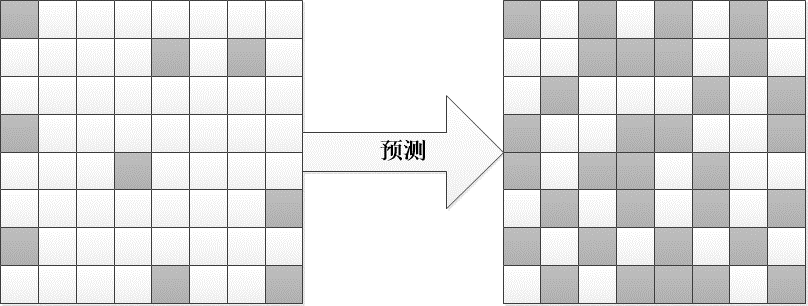
\includegraphics[scale=0.5]{fig/related_work/QoS_Prediction_Visualization.png}
			\caption{QoS预测问题形式化表达}
			\label{fig_QoS_Prediction_Visualization}
			\centering\zihao{5}{Fig 1.2 The cloud architecture}
		\end{figure}
		\section{基于协同过滤的QoS预测方法}
		\label{sec_QoS_Prediction_based_CF}
		
		\section{多目标(此处待定)}
		\label{sec_MultiObject}